% vqa.tex

% definition
With the goal of optimizing learning computations using quantum computers in
mind, we need an abstract idea of how to implement this connection. A
\emph{Variational Quantum Algorithm} (VQA) is any such system based on a
proposed architecture for a classically controlled quantum computer
\cite{bharti2021noisy}. \autoref{fig:vqaarch} presents the proposed
architecture. The following subsection presents an expanded view of the
computation.

% hybrid diagram
\begin{figure}
    \centering
    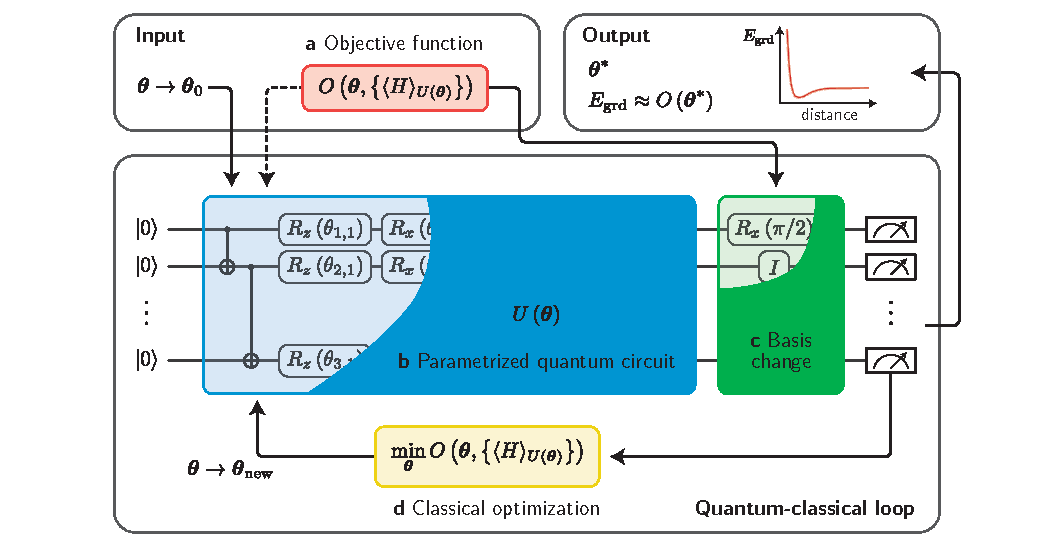
\includegraphics[width=\textwidth]{figures/vqaarch.pdf}
    \caption{Diagrammatic representation of a Variational Quantum Algorithm
    (VQA) \cite[see][chapter 3]{bharti2021noisy}.}
    \label{fig:vqaarch}
\end{figure}


\subsection{Building Blocks}

A VQA computation has 4 major components, as shown in \autoref{fig:vqaarch}:

\begin{itemize}
    \item objective function --- the encoding of the problem at hand as an
            optimization,
    \item parametrized quantum circuit (PQC) --- circuit encoding a unitary
            operator parametrized by classically controlled parameters
            \(\vec{\theta}\),
    \item measurement scheme --- the system performing basis changes and
            transferring outputs to the control system, and
    \item classical optimizer --- a classical objective minimizer which controls
            the PQC.
\end{itemize}

These components form a modular computation model where each of the components
can be swapped and improved individually to relieve bottnecks and adapt to the
problem at hand, to control the expressiveness of the system or avoid
treacherous optimization landscapes \cite{larocca2021theory}.

\subsubsection{Objective Function}

\subsubsection{Parametrised Quantum Circuits}
% pqc
% expressiveness of pqc
Expressiveness \cite{larocca2021theory}.

\subsubsection{Measurement}

\subsubsection{Parameter Optimisation}